
\chapter{進化論}



\section{ダーウィン『種の起源』 (1859)}



典拠:ダーウィン、八杉龍一訳(1990)『種の起源(上)』岩波書店

\subsection{}



つぎのこともまた、問われるであろう。私が発端の種とよんだ変種は、いかにしてついに、十分に資格のあるはっきりした種、つまり大部分の場合には同種の変種どうしよりも相互にずっと多くの差異を示すことが明らかなものである種に、変わっていくのであろうか。ちがった属とよばれるものの成員とされ、同属の種どうしよりも相互に多くの差異を示す種の群は、いかにして生じるのであろうか。これらのことはすべて、次章でさらにくわしくのべるように、生活のための闘争の結果として生じるのである。この生活のための闘争によって、変異は、いかに軽微なものであっても、またどんな原因から生じたものでも、どの種でもその一個体にいくらかでも利益になるものであったら、他の生物および外的自然に対する無限に複雑な関係において、その個体を保存させるようにはたらき、そして一般に子孫に受けつがれていくであろう。子孫もまた、これと同様に、生存の機会をよりめぐまれやすくなる。というのは、どの種でも周期的に多数の子がうまれるが、そのうち少数のものだけが存続していかれるからである。どんな軽微な変異も有用であれば保存されていくというこの原理を、それと人間の選択の力との関係をあらわすために、私は〈自然選択〉の語でよぶことにした。人間が選択によって確実に大きな結果を生ぜしめうること、また〈自然〉の手がかれにあたえた、軽微ではあるが有用な変異の集積により、生物を自分の用途に適応させていかれることについては、すでにのべた。しかし自然選択は、のちに明らかになるように、いつでもはたらけるように用意されている力であり、しかも人間の弱小な努力とはまったく比較にならない大きさのもので、それは〈自然〉の仕事が〈人工〉の作品にたいするのと同様である。(86-87)

\subsection{}


私は〈生存闘争〉という言葉を、ある生物が他の生物に依存するということや、個体が生きていくことだけでなく子孫をのこすに成功すること(これはいっそう重要なことである)をふくませ、広義に、また比喩的な意味に、もちいるということを、あらかじめいっておかねばならない。飢餓におそわれた二頭の肉食獣は、食物をえて生きるためにたがいに闘争するといわれてよいことは、たしかである。しかし砂漠のへりに生育している一本の植物も、乾燥にたいして生活のための闘争をしているといわれる。ただ、これは正しくいえば、湿度に依存しているのである。年ごとに千粒の種子を生じ、平均してそのうち一つだけが成熟する植物では、すでに地上をおおっている同種類または異種類の植物と闘争しているということが、前の場合よりもたしかにいえるであろう。〔……〕

生存闘争は、あらゆる生物が高率で増加する傾向をもつことの不可避的な結果である。すべての生物はそのほんらいの寿命のあいだに多数の卵あるいは種子を生じるものであるが、一生のある時期に、ある季節あるいはある年に、ほろびねばならない。もしそうでなければ、幾何学的〔等比数列的〕増加の原則によって、その個体数はたちまち法外に増大し、どんな国でもそれを収容できなくなる。このように生存の可能な以上に多くの個体がうまれるので、あらゆる場合に、ある個体と同種の他の個体との、あるいはちがった種の個体との、さらにまた生活の物理的条件との、生存闘争が当然生じることになる。これは、マルサスの学説を全動植物界にたいし何倍もの力で適用したものである。なぜなら、この場合には、食物の人為的な増加もなく、結婚の用心ぶかい制限もありえないからである。現在多少とも個体数がふえている種もあるが、すべての種がそうであるわけにはいかない。この世界がそれを保持することはできないのである。(88-90)


  \begin{figure}[htbp]
    \centering
      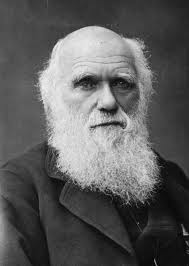
\includegraphics[width=50mm]{images/darwin.jpg}
      \caption{ダーウィン} 

  \end{figure}



\section{ダーウィン『人間の進化と性淘汰』 (1871)}



典拠:チャールズ・ロバート・ダーウィン、長谷川眞理子訳(1999)『ダーウィン著作集1 人間の進化と性淘汰』文一総合出版


\subsection{}


人間に関する新しい事実は、本書にはほとんど含まれていない。しかし、おおまかな原稿を書いたあとで私が到達した結論は興味あるものに見えたので、他の人々もおそらく興味を覚えるだろうと私は考えた。人間の起源については、決してわかることはないだろうと、しばしば自信を持って主張されてきた。しかし、知識よりも無知の方が、より多くの自信を生み出すものだ。あれやこれやの問題が、科学によって解けることは決してないだろうと強く主張するのは、より多くを知っている人たちではなく、より少なくしか知らない人たちである。人間が、他の種とともに、古くて、下等で、今は絶滅してしまった何らかの形態のものから由来したのだという結論は、決して新しいものではない。ラマルク(Lamarck)は、ずいぶん昔に同じ結論に達しているし、ウォレス(Wallace)、ハックスレイ、ライエル、フォークト、ラボック、ビュヒナー(Dr. Büchner)、ロル(Rolle)など、そして特にヘッケル(Häckel)といった著名な博物学者や哲学者も、近年、同じような考えを持つに至っている。(15)

\subsection{}


以下の提言は、大いに正しいであろうと私には思われる。すなわち、よく発達した社会的本能を備えた動物ならば、それがどんな動物であれ、その知的能力が人間のそれと匹敵するほどに発達すればすぐに、必然的に道徳観念または良心を提供するだろうということだ。なぜなら、まず第一に、社会的本能は、動物に、仲間と一緒の社会にいることに喜びを感じさせ、仲間に対していくらかの共感を抱かせ、彼らにさまざまな奉仕をさせるように導く。奉仕は、決まり切った、明らかに本能的な性質のもののこともあれば、多くの高等な社会的動物においてそうであるように、一般的な意味で自分の仲間を助けたいという望みや傾向であることもある。しかし、これらの感情や奉仕は、同種に属するすべての個体に対して振りまかれるものでは決してなく、いつも暮らしをともにしている個体に対してのみ向けられる。第二に、心的能力が高度に発達するやいなや、各個体の頭の中には、過去の行為や動機のイメージが絶え間なくよぎるようになるだろう。そして、これから見ていくように、常に底流に根強く存在している社会的本能が、一時的には強力だが常に存在するものではなく、あとに鮮烈な印象を残すわけでもないような他の本能に負けてしまったと感じたときにはいつでも、本能が充足されないときに生じるあの不満足感が起こるものだ。たとえば空腹時に感じるような多くの本能的欲求は短期のものであり、それが満たされてしまうと、すぐまた生き生きと思い出されるような性質のものではないことは明らかだ。第三に、言語の能力が獲得され、同じ社会に属するメンバーの要求がはっきりと表現されるようになったあとには、公共の善のためにそれぞれ何をするべきかに関する共通意見が、当然、行動の指針の大部分を占めるようになるに違いない。それでも依然として、社会的本能は社会の善のために行動する衝動を与えるだろうが、公共の意見がこの衝動を強め、方向づけ、ときには方向を変えさせることもあるだろう。この力は、これから見ていくように、本能的な共感に基づくのである。最後に、それぞれの個体がそのように行動するかの指針としては、究極的に個体の習慣が大きな役割を果たすに違いない。というのは、社会的本能や衝動も、他のすべての本能と同じく、習慣によって強化されるものであり、公共の意志や判断に従うかどうかということもそうだからだ。(70-71)

\subsection{}


では次に、社会的および道徳的能力について検討してみよう。原始人または類人猿的な祖先が社会的になるためには、彼は他の動物を集団で暮らすように仕向けているのと同じような本能的感情を獲得せねばならなかったはずだ。そして、同様な一般的な性向を示したに違いない。彼らは、仲間に対して何らかの愛情を感じ、仲間から引き離されると不安に陥っただろう。彼らはたがいに危険を知らせあい、攻撃においても防御においても、たがいに助けあったことだろう。これらすべては、ある程度の共感、忠誠、そして勇気があったことを暗示するものである。このような社会的性質が、下等動物にとって何よりも重要であることを疑う者はいないが、人間の祖先においても同じようなやりかたで、つまり習性の遺伝に助けられた自然淘汰によって獲得されたことは明らかである。同じ地方に住んでいる原始人の二つの部族が競争することになり、(他の条件はすべて同じとして)一方の部族がいつでもたがいに危険を知らせあい助けあう用意のあるような、勇気と共感と誠実さとを備えた人間をより多く持っていたならば、この部族が他の部族を征服し、最も栄えるようになるだろうことは間違いない。常に戦争が絶えないような未開人の社会において、誠実さと勇気がどれほど重要であるか、注意しておくことにしよう。規律のとれた兵隊が、無規律の烏合の衆に勝るのは、主に誰もが仲間に感じている信頼のためである。バジェット氏(Mr. Bagehot)がよく示しているように、服従は最も価値の高いものである。なぜなら、どんな形態の政府であれ、ないよりはましだからだ。利己的で争いを好む人々は皆で集まらないだろうが、集まらなければ何も出てこない。先にあげた性質を多く備えている部族は、よく備えて他の部族に打ち勝つだろうが、過去の歴史から判断する限り、長い年月の間には、より高度な能力を備えた別の部族に負けてしまうだろう。こうして、社会的および道徳的能力は徐々に高められ、世界中に広がることになる。

しかし、同じ部族の範囲のなかで、そもそも多くのメンバーがどうやって社会的および道徳的能力を持つようになったのか、その基準はどうやって高められていったのだろうかということが疑問になるだろう。より共感的で慈愛に満ちた親の子どもや、仲間に対して最も誠実であるような親の子どもが、同じ部族のなかで利己的で信用のおけない親の子どもより数多く育てられたとは、非常に考えにくい。多くの未開人がそうであるように、自分の仲間を裏切るよりは自らの命を犠牲にするような人間は、その高貴な性質を受け継ぐ子孫をまったく残さないことがしばしばある。戦争でいつも最前線に立ち、仲間のために命を捧げる用意のあるような、最も勇敢な男性は、そうでない男性よりも、平均して多数が死んでしまうだろう。それゆえ(いまここでは、一つの部族が他の部族に打ち勝つことを問題にしているのではないことに注意)、このような資質に恵まれた男性の数、またそのような素晴らしい性質の標準が、自然淘汰を通して、すなわち最適者の生存を通して高められていくとは、非常に考えにくいだろう。
 どのような状況であったために、同じ部族に属する人間の中で、このような資質を備えた人間の数が増えていったのかは、明らかにするにはあまりにも複雑であるかもしれないが、可能な段階のいくつかをたどることはできるだろう。まず第一に、各メンバーの推論の力と予測の力とが向上してくるにつれ、各自は自分の経験から、誰かを助ければふつうはお返しを得るということを素早く学習するに違いない。このような下賤な理由から、人間は仲間を助ける習慣を身につけるだろう。そして、仲間に対して慈愛に満ちた行動を取る習慣が、最初に慈愛に満ちた行動を取らせる衝動を与えているところの共感の感情をさらに強めることになったに違いない。そして、何世代にもわたって従われてきた習慣は、遺伝するようになるのだろう。

しかし、社会的道徳の発達を促した、もっとずっと強力な刺激がある。それは、仲間からの称賛と非難である。称賛を好み不名誉を嫌うことは、賞賛や非難をずっと記憶に保ち続けることとともに、第3章で検討した通り、主に共感の本能に基づいている。そしてこの本能も、他の社会的本能と同様に、自然淘汰によって獲得されたものに違いない。人間の進化の過程で、人間の祖先がどれほど早くから、仲間の賞賛や非難に動かされるような感情を持つようになったのかは、もちろん誰にもわからない。しかし、イヌでさえも、激励、称賛、非難がわかるようだ。最も粗野な未開人も、自分の武勇を示す戦利品を保存したり、過度に自慢したり、自分自身に外見や装飾に非常に気を使ったりすることにはっきりと表されているように、栄光という感情を持っている。彼らが仲間の意見を本当に気にかけているのでない限り、このような習慣には意味がないことだろう。(142-144)

\subsection{}


 道徳性の高さは、特定の一個人やその子どもたちを、同じ部族の他のメンバーに比べて、ほとんど、またはまったく有利にするものではないが、道徳の水準が上がり、そのような性質を備えた人物の数が増えれば、その部族が他の部族に対して非常に有利になるだろうということは忘れてはならない。愛国心、忠誠、従順、勇気、そして共感の感情をより高く保持していて、たがいに助け合ったり、全員の利益のために自分を犠牲にする用意のあるような人物をたくさん擁している部族が、他の部族に打ち勝つだろうことは間違いない。そして、これは自然淘汰である。いつの時代にも、世界のどこでも、ある部族が他の部族に置きかわってきた。そして、道徳は彼らの成功の一要因であるので、世界のどこでも道徳の標準は向上し、よりよい道徳を身につけた人間の数が増加したのである。(145)

\newpage{}

\section{ハクスリー『進化と倫理』(1894)}

出典:ジェームズ・パラディス、ジョージ・C・ウィリアムズ(編)『進化と倫理:トマス・ハクスリーの進化思想』、小林傳司・小川眞理子・吉岡栄二訳、産業図書、1995。

\subsection{}



哲学や宗教の問題についてはいかに見解が違っていても、人生における善悪の割合が人間の行為によって非常に大きな影響を受けるということについては大部分の人が同意していると仮定しても、さほど誤りではないと思うのです。私は、人間の行為によって悪が増えたり減ったりするということを疑う人を見たことがないのです。それゆえ、善も同様に増えたり減ったりするものであることになりそうです。結局、私の知る限りでは、われわれが物事を改善する能力を持っている限り、われわれ人類の最高の奉仕のために知力や活力を鍛錬することが、われわれの最高の責務だということを公然と疑う人を見たことがないのです。

そこでわれわれの当面の感心は、自然知識に関する現代の進歩、とりわけ進化論における進歩から引き出される一般的帰結が、相互扶助という偉大な仕事においてどの程度われわれの助けになってくれるのか、ということになるのです。

「倫理の進化」の方が彼らの思索を表現するのにふさわしいのに、「進化の倫理」と呼ばれるものを説く人々がいますが、彼らは道徳的感情が他の自然現象と同じく進化過程から生まれたものであるという主張をするために都合の良い、多かれ少なかれ興味深い事実や、それなりにまともな論証を引き合いに出しています。私の立場からすれば、彼らが正しい道を歩んでいることを疑っているわけではありません。ただ、不道徳感情も同じように進化してきたのですから、これもまた自然の承認を受けている点では変わりはないわけです。泥棒や人殺しも慈善家と同じように自然に従っているのえす。宇宙進化は人間の良き傾向や悪しき傾向がどのように生まれてきたかを告げてくれるかもしれませんが、宇宙進化自体は、善と呼ばれるものが悪と呼ばれるものよりもなぜ好ましいかということについては、従来われわれが手にしていたものより優れた理由を提供する力を持ってはいないのです。いつの日か、われわれが審美能力の進化を理解するときがきっとくるでしょう。しかし世界中の理解能力を集めても、これが美しく、あれは醜いといった直観の力を増やしたり減らしたりすることはないでしょう。

  \begin{figure}[htbp]
    \centering
      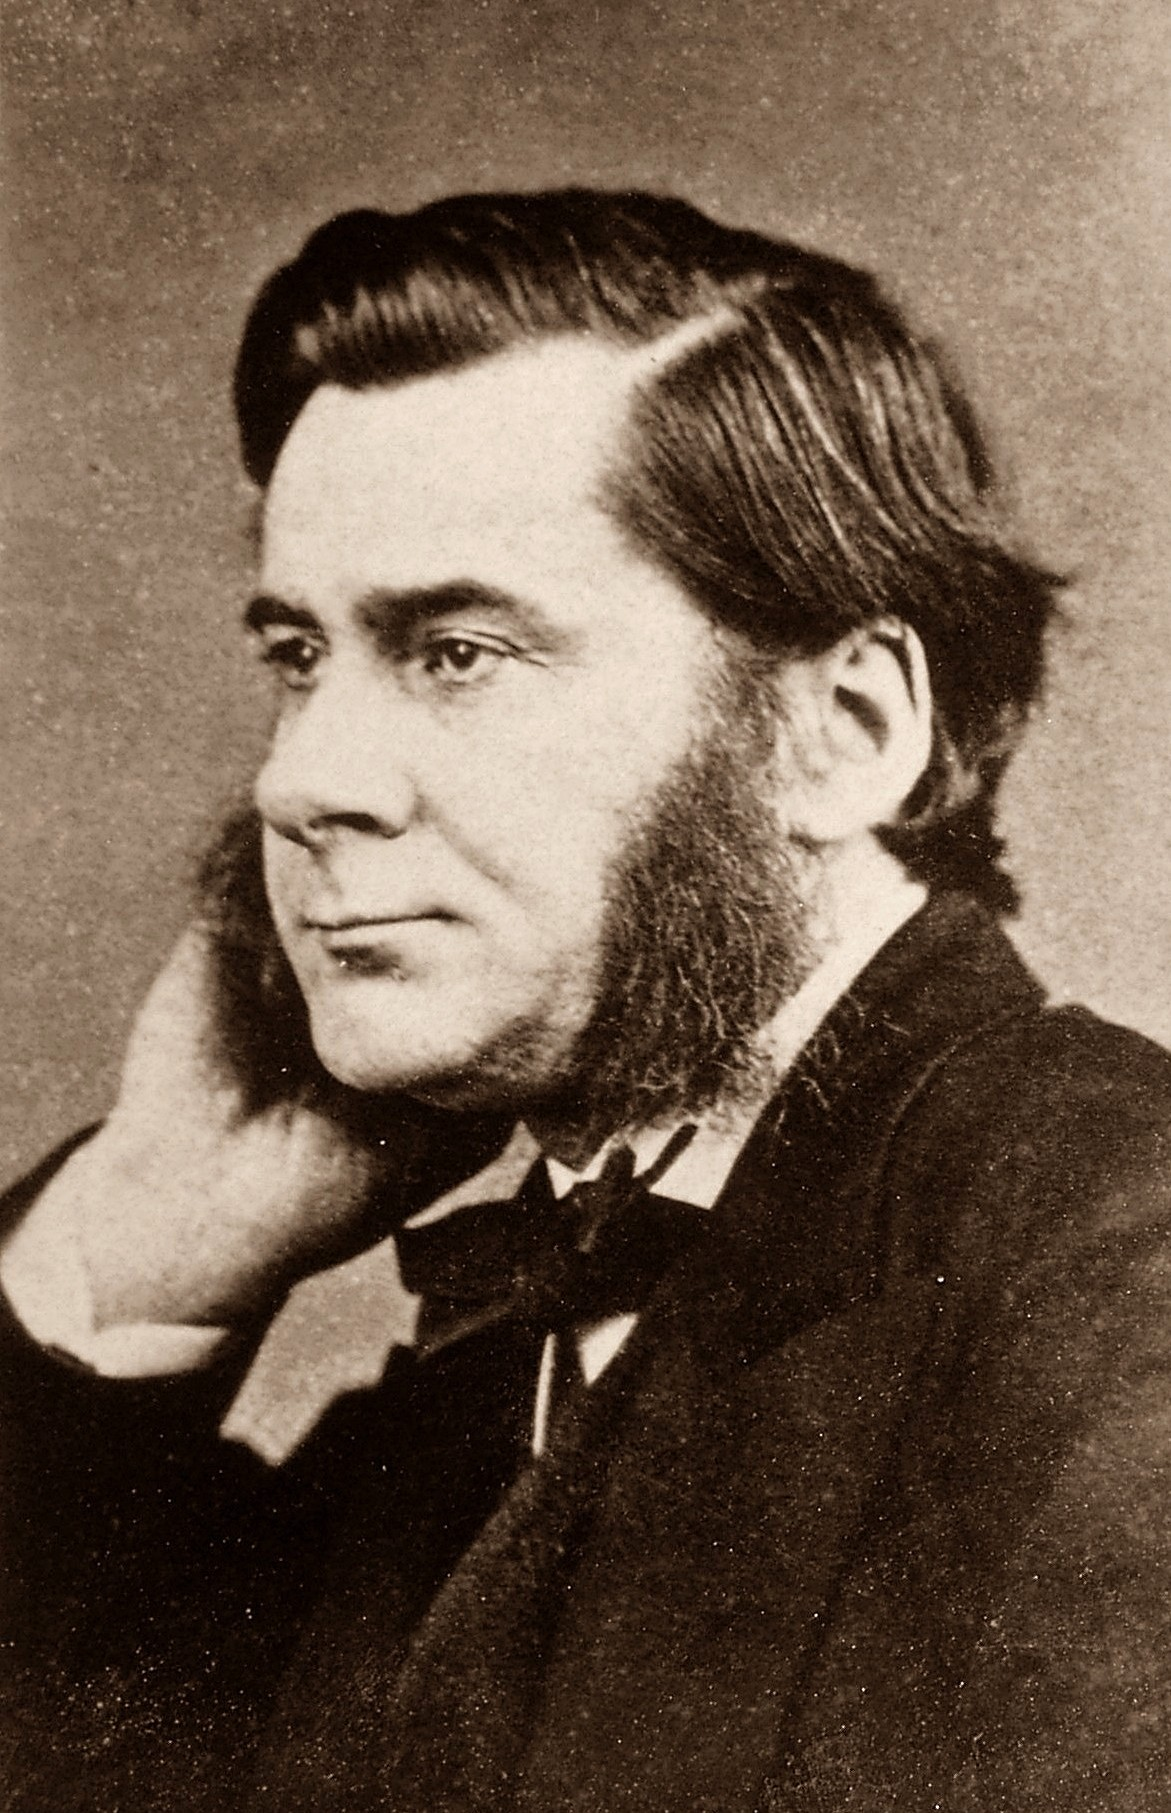
\includegraphics[width=50mm]{images/huxley.jpg}
    \caption{ハクスレー}
  \end{figure}


「進化の倫理」につきまとっていると思われるもう一つの誤りがあります。それは、全体としてみた場合、動物と植物は生存競争とその結果である「最適者生存」とによって、その有機組織の完成を進めていくのであるから、社会の中の人間、すなわち倫理的存在としての人間も自らの完成のために、それと同じ過程の助けを揉めねばならないという考え方です。私はこの誤りが生まれたのは「最適者生存」という用語が不幸にも曖昧だったからではないかと思います。「最適者」という言葉には、「最良」という含みがあります。そして「最良」という言葉には道徳的な香りがつきまおいます。しかし宇宙という自然においては、何が「最適者」であるかは条件次第です。ずっと以前に指摘したように、われあれの半球が復び冷暖化することがあれば、最適者生存の原理は植物界に、次第にいじけたお粗末な有機体の一群をもたらし、生き残った「最適者」は地衣類、珪藻類や雪を赤く染めるような微小な生物の他にはいなくなってしまうでしょう。一方、もし温暖化すれば、テムズ河やその上流のアイシス河の快適な渓谷は、熱帯のジャングルに生息する生物以外にどんな生物も住めなくなってしまうでしょう。最適者としての彼らは変化した環境に一番うまく順応したために、生き残ることになるでしょう。

社会の中の人間が、宇宙過程に従属することは疑う余地がありません。他の動物と同じく、繁殖は休むことなく行なわれ、それが必然的に生命維持のための烈しい競争をひきおこしています。この生存競争は、その生存する環境に自分をもっともうまく順応させる力をもっていないものを取り除いていきます。もっとも強いもの、もっとも自己主張の強いものが弱いものを踏みにじる傾向にあります。しかし、社会の進化に及ぼす宇宙過程の影響が強ければ強いほど、その社会の文明は用地なのです。社会の進歩とは、宇宙過程を一歩ごとに押さえつけ「倫理過程」とでも呼びうる別のものによって置き換えていくことなのです。そしてこの過程の目的は、とりあえず存在している諸条件の全体に関してたまたま最適者であるものを生き残らせるということではなく、倫理的に最良のものを生き残らせることなのです。

さきに主張しておいたように、倫理的に一番優れたこと{\——}すなわちわれわれが善あるいは徳と呼ぶもの{\——}を実践するには、宇宙的な生存競争において成功をおさめるものとはあらゆる点で対立する行動の道筋をとらなければなりません。このような実践は、無慈悲な自己主張のかわりに、一人一人が同胞を尊敬するだけでなく、助け合うことを要求するのです。その力は最適者の生存にではなく、できる限り多くの人を生き残るに的したものにすることに向けられるのです。この実践は、生存のための血で血を洗う競争という考え方を退けます。また、公共社会を苦労して作り上げてきた人々に対する自分の負い目を忘れず、自分が生存を許されている組織を自らの行為によって弱めることのないように要求するのです。法律は道徳律は宇宙過程を抑え、一人一人に自らの共同体に対する責務を思い起こさせるという目的に向けられているのです。(156-157)



\vspace{2zw}
\section{推薦図書}



\begin{itemize}
\item 内井惣七(2009)『ダーウィンの思想:人間と動物のあいだ』岩波書店。エッジのたった新書。ダーウィン思想のどこか革新的なのかがよくわかる。(渡)
\item ピエール・ダルモン (1992) 『医者と殺人者:ロンブローゾと生来性犯罪者伝説』、新評論。19世紀後半の生物学の発展などを受けて犯罪などに対する考え方も変り、「犯罪学」が成立する。そうした新しい思想はさまざまな問題を含んでいた。ロンブローゾはそうした立役者の一人。(江)
\end{itemize}


%%% Local Variables:
%%% mode: japanese-latex
%%% TeX-master: "main_gendai"
%%% coding: utf-8
%%% End:
